%package list
\documentclass{article}
\usepackage[top=3cm, bottom=3cm, outer=3cm, inner=3cm]{geometry}
\usepackage{graphicx}
\usepackage{url}
%\usepackage{cite}
\usepackage{hyperref}
\usepackage{array}
\usepackage{multicol}
\newcolumntype{x}[1]{>{\centering\arraybackslash\hspace{0pt}}p{#1}}
\usepackage{natbib}
\usepackage{pdfpages}
\usepackage{multirow}
\usepackage{float}
\usepackage[normalem]{ulem}
\useunder{\uline}{\ul}{}
\usepackage{svg}
\usepackage{amsmath}  
\usepackage{hyperref}
  
%%%%%%%%%%%%%%%%%%%%%%%%%%%%%%%%%%%%%%%%%%%%%%%%%%%%%%%%%%%%%%%%%%%%%%%%%%%%
%%%%%%%%%%%%%%%%%%%%%%%%%%%%%%%%%%%%%%%%%%%%%%%%%%%%%%%%%%%%%%%%%%%%%%%%%%%%
\newcommand{\csemail}{vmachacaa@unsa.edu.pe}
\newcommand{\csdocente}{Vicente Machaca Arceda}
\newcommand{\cscurso}{Algoritmos y Estructura de Datos}
\newcommand{\csuniversidad}{Universidad Nacional de San Agustín}
\newcommand{\csescuela}{Maestría en Ciencias de la Computación}
\newcommand{\cspracnr}{02}
\newcommand{\cstema}{--}
%%%%%%%%%%%%%%%%%%%%%%%%%%%%%%%%%%%%%%%%%%%%%%%%%%%%%%%%%%%%%%%%%%%%%%%%%%%%
%%%%%%%%%%%%%%%%%%%%%%%%%%%%%%%%%%%%%%%%%%%%%%%%%%%%%%%%%%%%%%%%%%%%%%%%%%%%


\usepackage[english,spanish]{babel}
\usepackage[utf8]{inputenc}
\AtBeginDocument{\selectlanguage{spanish}}
\renewcommand{\figurename}{Figura}
\renewcommand{\refname}{Referencias}
\renewcommand{\tablename}{Tabla} %esto no funciona cuando se usa babel
\AtBeginDocument{%
	\renewcommand\tablename{Tabla}
}

\usepackage{fancyhdr}
\pagestyle{fancy}
\fancyhf{}
\setlength{\headheight}{30pt}
\renewcommand{\headrulewidth}{1pt}
\renewcommand{\footrulewidth}{1pt}
\fancyhead[L]{\raisebox{-0.2\height}{
\includegraphics[width=3cm]{img/logo_unsa}}}
\fancyhead[C]{}
\fancyhead[R]{\fontsize{7}{7}\selectfont	\csuniversidad \\ \csescuela \\ \textbf{\cscurso} }
\fancyfoot[L]{Grupo N° 02}
\fancyfoot[C]{\cscurso}
\fancyfoot[R]{Página \thepage}


\begin{document}
	
	\vspace*{10px}
	
	\begin{center}	
		\fontsize{17}{17} \textbf{ Práctica \cspracnr}
	\end{center}
	%\centerline{\textbf{\underline{\Large Título: Informe de revisión del estado del arte}}}
	%\vspace*{0.5cm}
	

	\begin{table}[h]
		\begin{tabular}{|x{4.7cm}|x{4.8cm}|x{4.8cm}|}
			\hline
			\textbf{DOCENTE} & \textbf{CARRERA}  & \textbf{CURSO}   \\
			\hline
			\csdocente & \csescuela & \cscurso    \\
			\hline
		\end{tabular}
	\end{table}	
	
	
	\begin{table}[h]
		\begin{tabular}{|x{4.7cm}|x{4.8cm}|x{4.8cm}|}
			\hline
			\textbf{PRÁCTICA} & \textbf{TEMA}  & \textbf{DURACIÓN}   \\
			\hline
			\cspracnr & \cstema & --   \\
			\hline
		\end{tabular}
	\end{table}
	
	\section{Integrantes}
        	\begin{itemize}
        		\item Grupo N° 2
        		\item Integrantes:
        		\begin{itemize}
        			\item EDER ALONSO AMPUERO ATAMARI
        			\item HOWARD FERNANDO ARANZAMENDI MORALES
        			\item JOSE EDISON PEREZ MAMANI
        			\item HENRRY IVAN ARIAS MAMANI
        		\end{itemize}		
        	\end{itemize}
    \section{Repositorio GitHub}
           URL Github: \href{https://github.com/hAriasm/Practica2_ayed}{Repositorio Práctica 2 AyED}
	\section{Estructuras de Datos}
        \subsection{BTree}
            \paragraph{}
   zzzzzzzzzz


        \subsection{AVL}

         El Merge Sort es un algoritmo recursivo bastante eficiente para ordenar un array, que tiene un orden de complejidad O(nlogn) al igual que Quick Sort. fue desarrollado en 1945 por John Von Neumann.

         El Merge Sort está basado en la técnica de diseño de algoritmos Divide y Vencerás, esta técnica consiste en dividir el problema a resolver en sub problemas del mismo tipo que a su vez se dividirán, mientras no sean suficientemente  pequeños o triviales Figura
         
         \subsubsection{Resultados del experimento}
         \begin{itemize}
           \item En la figura \ref{fig:avlInicial} mostramos nuestro árbol inicial con 11 nodos.
           \item En la figura \ref{fig:avlIsertion} mostramos el árbol luego de insertar un nodo nuevo.
           \item En la figura \ref{fig:avldelete} mostramos luego de eliminar un nodo.
           \item En la figura \ref{fig:avldelete2} mostramos luego de eliminar el nodo raíz.
         \end{itemize}
 
            \begin{figure}[htbp]
              \centering
              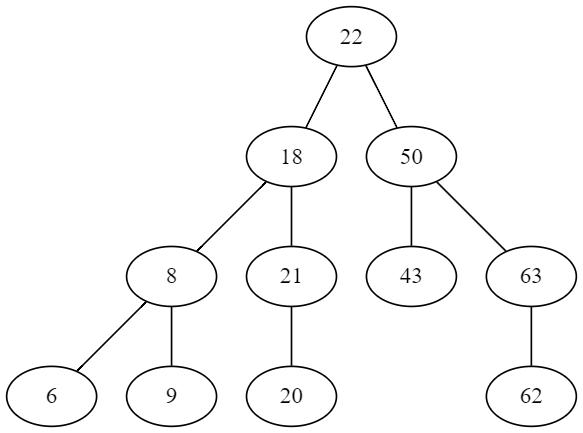
\includegraphics[width=0.5\textwidth]{img/avltree.png}
              \caption{Árbol AVL inicial}
              \label{fig:avlInicial}
            \end{figure}
            \begin{figure}[htbp]
              \centering
              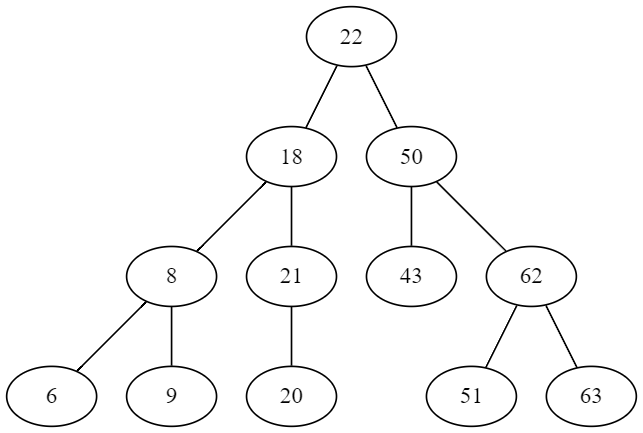
\includegraphics[width=0.5\textwidth]{img/avltree-insertion.png}
              \caption{Árbol AVL con inserción }
                \label{fig:avlIsertion}
            \end{figure}
            \begin{figure}[htbp]
              \centering
              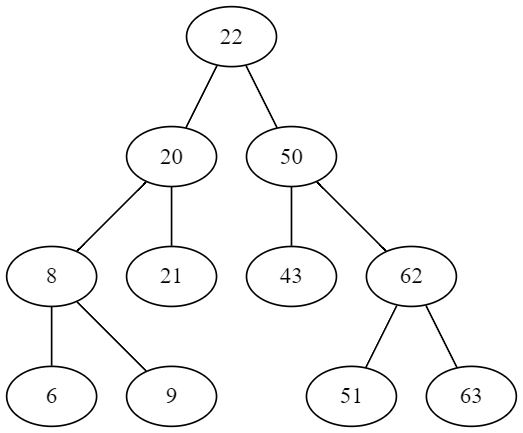
\includegraphics[width=0.5\textwidth]{img/avltree-deletion.png}
              \caption{Árbol AVL con eliminación nodo}
            \label{fig:avldelete}
            \end{figure}
             \begin{figure}[htbp]
              \centering
              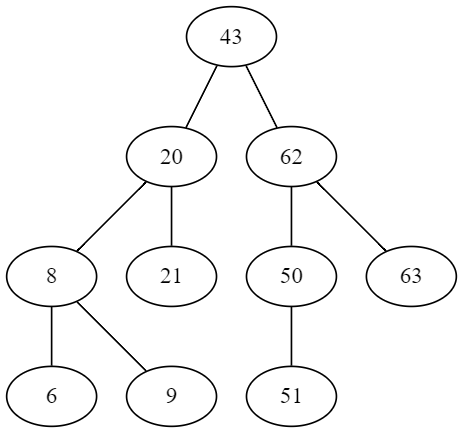
\includegraphics[width=0.5\textwidth]{img/avltree-deletion-2.png}
              \caption{Árbol AVL con eliminación de la raíz}
              \label{fig:avldelete2}
            \end{figure}

    \section{Conclusiones}
        \begin{itemize}
                 \item  ssss
                 \item	ssss
                 \item Un árbol AVL se mantiene ordenado, pero hay mas rotaciones en las inserciones que en las eliminaciones, su costo para buscar, eliminar, insertar  es de O(Log n).
                 \item  
        \end{itemize}

    \section{Referencias}
  

\end{document} 